\documentclass[11pt, a4paper]{article}

% 한국어 패키지
\usepackage{kotex}
\usepackage[utf8]{inputenc}

% 기본 패키지
\usepackage{graphicx}
\usepackage{amsmath}
\usepackage{amssymb}
\usepackage{hyperref}
\usepackage{listings}
\usepackage{xcolor}
\usepackage{geometry}
\usepackage{setspace}
\usepackage{titlesec}
\usepackage{fancyhdr}
\usepackage{caption}
\usepackage{subcaption}
\usepackage{booktabs}
\usepackage{float}

% 페이지 설정
\geometry{
    top=25mm,
    bottom=25mm,
    left=25mm,
    right=25mm
}

% 코드 스타일 설정
\lstset{
    basicstyle=\ttfamily\small,
    keywordstyle=\color{blue},
    commentstyle=\color{gray},
    stringstyle=\color{red},
    breaklines=true,
    frame=single,
    backgroundcolor=\color{gray!10},
    showstringspaces=false,
    tabsize=4
}

% 제목 형식 설정
\titleformat{\section}{\Large\bfseries}{\thesection.}{1em}{}
\titleformat{\subsection}{\large\bfseries}{\thesubsection.}{1em}{}
\titleformat{\subsubsection}{\normalsize\bfseries}{\thesubsubsection.}{1em}{}

% 줄간격 설정
\setstretch{1.3}

% 헤더 설정
\pagestyle{fancy}
\fancyhf{}
\fancyhead[L]{딥러닝 최종보고서}
\fancyhead[R]{2024193011 신재완}
\fancyfoot[C]{\thepage}

\begin{document}

% 제목 페이지
\begin{titlepage}
    \centering
    \vspace*{3cm}
    {\LARGE\bfseries 딥러닝 최종보고서}\\[2cm]
    {\Large 전체 Page의 배경과 캐릭터 일관성을 유지하는\\Manga Colorization 과 Translation}\\[3cm]
    {\large
    학번: 2024193011\\[0.5cm]
    이름: 신재완\\[2cm]
    }
    \vfill
    {\large 2025년 12월 8일}
\end{titlepage}

% 목차
\tableofcontents
\newpage

% 요약
\section*{요약}
\addcontentsline{toc}{section}{요약}

본 연구는 manga의 채색(colorization)과 번역(translation) 작업을 자동화하면서 전체 페이지에 걸쳐 배경과 캐릭터의 일관성을 유지하는 시스템을 구축하는 것을 목표로 한다. 기존의 line art colorization 모델인 MangaDiT와 MangaNinja는 높은 컴퓨팅 자원을 요구하거나 reference 이미지가 필수적이며, 여러 panel을 동시에 처리하는 데 한계가 있다. 본 연구에서는 Gemini Imagen 3 기반의 Nano Manana 시스템을 개발하여 이러한 한계를 극복하고자 하였다. 제안된 시스템은 batch 처리를 통해 번역 작업에서 최대 10배, 채색 작업에서 최대 5배의 속도 향상을 달성하였다. 또한 의성어, 의태어, 물체 내 텍스트를 포함한 이중 언어 번역과 그림자 및 빛 효과가 향상된 채색이 가능하다. 실험 결과, 대다수의 경우에서 높은 품질의 채색과 번역이 이루어졌으나, 원본에 없는 장면이 생성되거나 일관성이 무너지는 경우가 일부 존재하였다. 이러한 문제는 모델 자체의 특성에 기인하며, 향후 사용자 확인 기반의 재생성 기능을 통해 해결할 수 있을 것으로 기대된다.

\newpage

% 서론
\section{서론}

\subsection{연구 주제 소개}

Manga, cartoon, manhwa와 같은 작품을 제작할 때 채색 작업은 제작 시간을 2$\sim$3배 이상 증가시키는 주요 요인이다. 이러한 시간적 부담으로 인해 현재까지도 많은 manga 작품들이 흑백(monochrome) 형태로 출판되고 있다. 인공지능을 활용한 자동 채색 기술은 이러한 문제를 해결할 수 있는 유망한 접근법이지만, 다음과 같은 기술적 어려움이 존재한다.

\begin{figure}[H]
    \centering
    \includegraphics[width=0.8\textwidth]{figure/manga_difficulty_colorization_example.png}
    \caption{Manga 채색의 어려움 예시}
    \label{fig:colorization_difficulty}
\end{figure}

첫째, 캐릭터와 배경을 정확하게 구분하여 적절한 색상을 적용해야 한다. 둘째, 동일한 캐릭터가 여러 페이지에 걸쳐 등장할 때 눈 색깔, 머리카락 색, 피부색, 의상 색상 등의 일관성을 유지해야 한다. 셋째, 동일한 배경이나 물체가 반복적으로 등장할 때 색상의 일관성을 보장해야 한다. 넷째, manga 특유의 panel(칸) 구조를 손상시키지 않으면서 채색을 수행해야 한다.

\begin{figure}[H]
    \centering
    \includegraphics[width=0.8\textwidth]{figure/manga_difficulty_translation_example.png}
    \caption{Manga 번역의 어려움 예시}
    \label{fig:translation_difficulty}
\end{figure}

번역 작업 또한 상당한 시간과 노력이 필요한 분야이다. Manga 번역은 단순한 텍스트 번역 이상의 복잡성을 가진다. 일반적으로 역본 작업(텍스트를 번역하는 작업)과 식질 작업(번역된 텍스트를 이미지에 자연스럽게 삽입하는 작업)의 두 단계로 구성된다. AI를 활용한 자동 번역에서는 그림 속에 포함된 의성어와 의태어의 자연스러운 번역, 그리고 배경이나 물체에 포함된 텍스트의 일관된 번역이 주요 과제로 남아있다.

\subsection{연구의 중요성}

본 연구는 manga 제작 생태계에 실질적인 기여를 할 수 있는 잠재력을 가진다. 자동화된 채색 및 번역 시스템을 통해 manga 제작에 소요되는 시간을 대폭 단축하면서도 높은 품질을 유지할 수 있다. 이는 개인 창작자부터 출판사에 이르기까지 다양한 규모의 제작 주체들에게 혜택을 제공할 수 있다.

특히 번역 자동화는 manga의 글로벌 확산에 핵심적인 역할을 할 수 있다. 현재 대부분의 manga는 번역 비용과 시간의 제약으로 인해 일본 국내 시장에 한정되어 유통되고 있다~\cite{mangamllm}. 효과적인 자동 번역 시스템의 구축은 더 많은 언어권의 독자들이 다양한 manga 작품을 접할 수 있는 기회를 제공하며, 이는 manga 산업의 글로벌 성장을 촉진할 수 있다.

\subsection{결과 요약}

본 연구에서 개발한 Nano Manana 시스템은 다음과 같은 성과를 달성하였다. Batch 처리 구조를 통해 기존 순차적 처리 방식 대비 번역 작업에서 최대 10배, 채색 작업에서 최대 5배의 속도 향상을 이루었다. 프롬프트 엔지니어링을 통해 그림자와 빛 효과가 개선된 다채로운 채색 결과를 생성할 수 있었다. 또한 의성어, 의태어, 물체 내 텍스트를 포함한 포괄적인 번역이 가능하며, 이중 언어(bilingual) 표시 기능도 구현하였다.

실험 결과, 18페이지 분량의 manga에 대해 대다수의 페이지에서 높은 품질의 채색과 번역이 이루어졌다. 그러나 일부 페이지에서 원본에 없는 장면이 생성되거나 캐릭터 일관성이 무너지는 현상이 관찰되었다. 이러한 문제는 사용된 생성 모델 자체의 특성에 기인하며, 사용자 확인 기반의 재생성(rerun) 기능을 통해 보완할 수 있음을 확인하였다.

\newpage

% 관련 연구
\section{관련 연구}

\subsection{MangaDiT}

MangaDiT~\cite{mangadit}는 Qiu 등이 2025년에 발표한 line art colorization 모델로, Diffusion Transformer 구조에서 계층적 어텐션(Hierarchical Attention)을 활용하여 reference 이미지를 기반으로 line art를 채색하는 기술이다.

\begin{figure}[H]
    \centering
    \includegraphics[width=0.9\textwidth]{figure/manga_dit.png}
    \caption{MangaDiT 모델 구조}
    \label{fig:manga_dit}
\end{figure}

MangaDiT는 FLUX1.dev를 기반으로 하며, transformer 아키텍처를 사용한다. 이 모델은 reference 이미지의 색상 정보를 계층적 어텐션 메커니즘을 통해 target line art에 효과적으로 전달함으로써, 캐릭터의 색상 일관성을 유지하면서 고품질의 채색 결과를 생성한다. 학습에는 NVIDIA A100 80GB GPU가 사용되었다.

\begin{figure}[H]
    \centering
    \includegraphics[width=0.7\textwidth]{figure/manga_dit_install_failed.png}
    \caption{MangaDiT 설치 실패 화면}
    \label{fig:manga_dit_fail}
\end{figure}

본 연구에서 MangaDiT를 직접 실행해보고자 하였으나, 환경 변수 설정 및 conda 환경 버전 충돌 문제로 인해 수 시간의 시도에도 불구하고 설치에 실패하였다. 또한 MangaDiT는 높은 VRAM을 요구하여 일반적인 개인용 GPU(예: RTX 3070 8GB)로는 실행이 불가능하다.

본 연구에서 제안하는 Nano Manana와의 주요 차별점은 다음과 같다. 첫째, MangaDiT는 채색을 위해 reference 이미지가 필수적으로 요구되는 반면, Nano Manana는 reference 없이도 높은 품질의 채색이 가능하다. 둘째, MangaDiT는 단일 line art 캐릭터 처리에 최적화되어 있는 반면, Nano Manana는 여러 panel이 포함된 전체 manga 페이지를 입력으로 받아 처리할 수 있다.

\subsection{MangaNinja}

MangaNinja~\cite{manganinja}는 Liu 등이 2025년에 발표한 line art colorization 모델로, 정밀한 reference following을 통해 line art를 채색하는 기술이다.

\begin{figure}[H]
    \centering
    \includegraphics[width=0.9\textwidth]{figure/manga_ninja.png}
    \caption{MangaNinja 모델 구조}
    \label{fig:manga_ninja}
\end{figure}

MangaNinja는 Stable Diffusion 1.5를 기반으로 하며, reference 이미지의 색상과 스타일을 target line art에 정밀하게 적용하는 것을 목표로 한다. 이 모델은 NVIDIA A100 80GB GPU 8장을 사용하여 약 하루 동안 학습되었다. 공식 문서에 따르면 6GB VRAM으로도 inference가 가능하다고 명시되어 있어 직접 실험을 진행하였다.

\begin{figure}[H]
    \centering
    \begin{subfigure}[b]{0.45\textwidth}
        \centering
        \includegraphics[width=\textwidth]{figure/manga_ninja_try1.png}
        \caption{MangaNinja 시도 1}
        \label{fig:manga_ninja_try1}
    \end{subfigure}
    \hfill
    \begin{subfigure}[b]{0.45\textwidth}
        \centering
        \includegraphics[width=\textwidth]{figure/manga_ninja_try2.png}
        \caption{MangaNinja 시도 2}
        \label{fig:manga_ninja_try2}
    \end{subfigure}
    \caption{MangaNinja 실험 결과}
    \label{fig:manga_ninja_results}
\end{figure}

실험 결과, NVIDIA RTX 3070 8GB 환경에서 한 장의 이미지를 inference하는 데 약 30분이 소요되었다. 약 30GB 크기의 모델을 다운로드하여 실행한 결과, 단일 캐릭터에 대해서도 reference 이미지의 일관성 유지가 충분하지 않았다. 특히 여러 panel을 포함한 전체 manga 페이지를 입력으로 제공하면 이미지가 전체적으로 흐려지고 뭉개지는 현상이 발생하였다.

Nano Manana와의 차별점은 MangaDiT와 유사하다. MangaNinja 역시 reference 이미지가 필수적으로 요구되며, 단일 캐릭터 처리에 최적화되어 있어 여러 panel이 포함된 manga 페이지를 직접 처리하기 어렵다.

\subsection{Context-Informed Machine Translation of Manga using Multimodal Large Language Models}

Lippmann 등~\cite{mangamllm}이 2025년 COLING에서 발표한 연구는 multimodal large language model(MLLM)을 활용하여 manga 번역의 품질을 향상시키는 방법론을 제안한다.

\begin{figure}[H]
    \centering
    \includegraphics[width=0.8\textwidth]{figure/manga_mllm.png}
    \caption{Context-Informed Manga Translation 개요}
    \label{fig:manga_mllm}
\end{figure}

이 연구는 manga 번역이 일반적인 텍스트 번역보다 복잡한 이유로 시각적 요소가 번역 과정에서 모호성을 해소하는 데 필수적이라는 점을 강조한다. 저자들은 MLLM의 vision 컴포넌트를 활용하여 번역 품질을 개선하는 방법론을 제안하였으며, 번역 단위 크기(translation unit size)와 context 길이가 번역 품질에 미치는 영향을 분석하였다. 또한 token 효율적인 manga 번역 접근법을 제안하였다.

주요 기여로는 일본어-영어 번역에서 state-of-the-art 결과를 달성하였으며, 최초의 일본어-폴란드어 병렬 manga 번역 데이터셋을 공개하였다. 또한 다른 연구자들이 LLM의 manga 번역 성능을 벤치마킹할 수 있도록 오픈소스 소프트웨어 도구를 제공하였다.

본 연구에서 제안하는 Nano Manana와의 주요 차별점은 다음과 같다. Lippmann 등의 연구는 텍스트 번역에 집중하여 번역된 텍스트만을 출력으로 제공하는 반면, Nano Manana는 번역된 텍스트가 이미지에 직접 삽입된 결과물을 생성한다. 즉, 역본 작업과 식질 작업을 통합하여 end-to-end로 번역된 manga 이미지를 출력한다. 이를 통해 의성어, 의태어, 배경 텍스트 등 이미지와 밀접하게 결합된 텍스트 요소들도 자연스럽게 번역된 결과물을 얻을 수 있다.

\newpage

% 데이터
\section{데이터}

\subsection{데이터 수집 방법}

본 연구에서는 실험을 위한 manga 데이터를 pixiv 플랫폼에서 수집하였다. 데이터 수집에는 gallery-dl~\cite{galleryDL}을 사용하였다. gallery-dl은 다양한 이미지 호스팅 사이트에서 이미지 갤러리와 컬렉션을 다운로드할 수 있는 command-line 도구로, pixiv의 특정 게시물 페이지에서 manga 이미지를 효율적으로 다운로드할 수 있다.

수집된 데이터는 두 가지 manga 작품으로 구성되며, 각각 다른 특성을 가지고 있어 시스템의 다양한 측면을 평가하는 데 활용되었다.

\subsection{合コンに行ったら女がいなかった話}

첫 번째 실험 데이터는 蒼川なな(Aokawa Nana) 작가의 「合コンに行ったら女がいなかった話」(How I Attended an All-Guy's Mixer)~\cite{pixiv_goukon}이다. 이 작품은 pixiv에서 연재되고 있는 창작 manga로, 일본어로 작성되어 있다.

\begin{figure}[H]
    \centering
    \includegraphics[width=0.5\textwidth]{figure/136886858_p0.png}
    \caption{「合コンに行ったら女がいなかった話」 표지}
    \label{fig:pixiv1_cover}
\end{figure}

해당 작품은 총 18페이지로 구성되어 있으며, 전체가 흑백(monochrome)으로 제작되어 있다. 이러한 특성은 채색 시스템의 성능을 평가하기에 적합하다. 여러 캐릭터가 등장하며 다양한 배경과 상황이 묘사되어 있어, 캐릭터 및 배경 일관성 유지 능력을 종합적으로 테스트할 수 있다.

\subsection{神は友達が少ない}

두 번째 실험 데이터는 ピノ/エス(Pino/Esu) 작가의 「神は友達が少ない」(God Has Few Friends)~\cite{pixiv_kami}이다. 이 작품 역시 pixiv에서 공개된 창작 manga로, 일본어로 작성되어 있다.

\begin{figure}[H]
    \centering
    \includegraphics[width=0.5\textwidth]{figure/107422372_p0.png}
    \caption{「神は友達が少ない」 표지}
    \label{fig:pixiv2_cover}
\end{figure}

해당 작품은 총 15페이지로 구성되어 있으며, 컬러 표지 1페이지와 흑백 14페이지로 이루어져 있다. 특히 이 작품에는 Genshin Impact라는 게임의 캐릭터들이 등장한다. 이러한 널리 알려진 캐릭터를 포함한 데이터는 생성 모델이 사전 학습된 지식을 활용하여 캐릭터 일관성을 유지하는 능력을 평가하는 데 유용하다.

\newpage

% 연구 방법
\section{연구 방법}

\subsection{Baseline}

Baseline 시스템으로는 Gemini 웹 애플리케이션(\url{https://gemini.google.com/app})을 사용하여 수동으로 채색 및 번역 작업을 수행하는 방식을 채택하였다. 이 방식에서는 페이지 한 장을 처리하고 완료되면 다음 페이지를 순차적으로 처리하는 sequential한 접근법을 사용한다.

\begin{figure}[H]
    \centering
    \begin{subfigure}[b]{0.45\textwidth}
        \centering
        \includegraphics[width=\textwidth]{figure/baseline_translate_batch_structure.png}
        \caption{Baseline 번역 처리 구조}
        \label{fig:baseline_translate}
    \end{subfigure}
    \hfill
    \begin{subfigure}[b]{0.45\textwidth}
        \centering
        \includegraphics[width=\textwidth]{figure/baseline_colorization_batch_structure.png}
        \caption{Baseline 채색 처리 구조}
        \label{fig:baseline_colorization}
    \end{subfigure}
    \caption{Baseline 시스템의 처리 구조}
    \label{fig:baseline_structure}
\end{figure}

채색 일관성 유지를 위해 이전에 생성된 모든 colorized image를 reference로 전달하는 방식을 사용한다. 즉, $n$번째 페이지를 채색할 때는 1번부터 $n-1$번까지의 채색된 이미지를 모두 context로 제공한다. 이 방식은 일관성 유지에는 효과적이지만, 페이지 수가 증가함에 따라 처리 시간이 선형적으로 증가하는 단점이 있다.

\subsection{Nano Manana}

Nano Manana는 본 연구에서 개발한 manga 채색 및 번역 자동화 시스템이다. Gemini의 Imagen 3 모델을 기반으로 하며, batch 처리와 최적화된 프롬프트를 통해 baseline 대비 높은 효율성과 품질을 달성한다.

\subsubsection{Batch 구현}

Nano Manana의 핵심 설계 원칙은 효율적인 batch 처리를 통한 속도 향상이다. 번역과 채색 작업에 대해 각각 다른 batch 처리 전략을 적용하였다.

\begin{figure}[H]
    \centering
    \begin{subfigure}[b]{0.45\textwidth}
        \centering
        \includegraphics[width=\textwidth]{figure/nano_manana_translate_batch_structure.png}
        \caption{Nano Manana 번역 batch 구조}
        \label{fig:nano_translate_batch}
    \end{subfigure}
    \hfill
    \begin{subfigure}[b]{0.45\textwidth}
        \centering
        \includegraphics[width=\textwidth]{figure/nano_manana_colorization_batch_structure.png}
        \caption{Nano Manana 채색 batch 구조}
        \label{fig:nano_colorization_batch}
    \end{subfigure}
    \caption{Nano Manana 시스템의 batch 처리 구조}
    \label{fig:nano_batch_structure}
\end{figure}

번역 작업의 경우, \texttt{batch\_size}만큼의 페이지를 한 번에 병렬로 처리하고, 모든 페이지가 완료될 때까지 대기한 후 다음 batch를 처리한다. 번역은 각 페이지가 독립적으로 처리될 수 있으므로 완전한 병렬화가 가능하다.

채색 작업의 경우, 일관성 유지를 위해 이전에 완료된 페이지들을 reference로 활용해야 하므로 보다 복잡한 전략이 필요하다. 각 batch에서 $\min(\text{batchNumber}, \text{batchSize}, \text{completedCount})$개의 reference 이미지를 전달하고, 동일한 수의 output 이미지를 batch로 생성한다. 여기서 \texttt{batchNumber}는 현재 batch의 순번, \texttt{completedCount}는 현재까지 완료된 페이지 수를 의미한다. 첫 번째 batch에서는 \texttt{completedCount}가 0이므로 예외적으로 1을 사용한다.

\subsubsection{프롬프트 설계}

효과적인 프롬프트 설계는 생성 결과의 품질에 직접적인 영향을 미친다. 본 연구에서는 번역, 채색, 그리고 번역과 채색을 동시에 수행하는 세 가지 유형의 프롬프트를 설계하였다.

\paragraph{번역 프롬프트}
번역 프롬프트는 다음과 같은 핵심 지침을 포함한다.

\begin{lstlisting}[caption={번역 프롬프트 예시}]
Translate this manga page from Japanese to Korean. 

IMPORTANT TRANSLATION GUIDELINES:
- Do NOT translate literally word-by-word. Instead, think about 
  the context, character emotions, and scene atmosphere.
- Adapt the translation to sound natural in Korean while 
  preserving the original meaning and tone.
- Consider manga-specific expressions, onomatopoeia, and cultural 
  nuances when translating.
- Make the dialogue flow naturally as if it was originally 
  written in Korean.

IMAGE REQUIREMENTS:
- Maintain all characters, backgrounds, speech balloon shapes, 
  panel grids, and manga structure.
- The original image size is 2129x3000. Make image which has 
  EXACTLY SAME ratio and layout with original one.
- Translate speech balloon text, onomatopoeia, handwritten text, 
  and all other texts that are not in Korean.
- Keep all visual elements unchanged except for the translated text.
\end{lstlisting}

번역 프롬프트에서는 단순한 직역이 아닌 맥락과 감정을 고려한 자연스러운 번역을 유도한다. 또한 원본 이미지의 비율과 레이아웃을 정확히 유지하도록 명시하여 출력 이미지의 품질을 보장한다.

\paragraph{채색 프롬프트}
채색 프롬프트는 첫 번째 페이지와 이후 페이지에 대해 다른 구조를 가진다. 첫 번째 페이지에서는 reference 없이 채색을 수행하고, 이후 페이지에서는 이전에 채색된 페이지들을 reference로 제공한다.

\begin{lstlisting}[caption={채색 프롬프트 예시 (첫 번째 페이지)}]
Colorize the manga page below. Refer to no reference images to 
maintain consistency in character eye color, skin color, hair 
color, and clothing color.

COLORING STYLE REQUIREMENTS:
- Apply vibrant, rich, and diverse colors throughout the entire 
  image.
- Do NOT leave any area uncolored - fill every part with 
  appropriate colors including backgrounds, objects, and small 
  details.
- Use a colorful and visually appealing palette that brings the 
  manga to life.
- Add depth and dimension with shading and highlights where 
  appropriate.
- Make the coloring look professional and polished like a 
  published color manga.

CONSISTENCY REQUIREMENTS:
- Maintain consistency for the same character, but if the 
  character is wearing new clothing, draw them with appropriate 
  different clothing.
- Maintain cosmetic features (eye color, hair color, skin tone) 
  consistently for each character across all pages.
\end{lstlisting}

여러 reference를 사용하는 경우, 프롬프트 앞부분에 다음과 같이 reference 이미지들을 명시한다.

\begin{lstlisting}[caption={채색 프롬프트 예시 (reference 사용)}]
This is reference page 1 (already colorized):
[Image: page1]

This is reference page 2 (already colorized):
[Image: page2]

Colorize page 3:
[Image: page3]

Colorize the manga page below. ...
\end{lstlisting}

\paragraph{채색 및 번역 통합 프롬프트}
채색과 번역을 동시에 수행하는 프롬프트는 위의 두 프롬프트의 요소를 통합하여 구성한다. 이를 통해 한 번의 API 호출로 두 가지 작업을 동시에 수행할 수 있어 효율성이 향상된다.

\subsubsection{이중 언어 표시}

Nano Manana는 이중 언어(bilingual) 표시 기능을 지원한다. 이 기능은 원본 언어와 번역된 언어를 동시에 표시하여, 언어 학습이나 번역 검증에 유용하게 활용될 수 있다.

\begin{figure}[H]
    \centering
    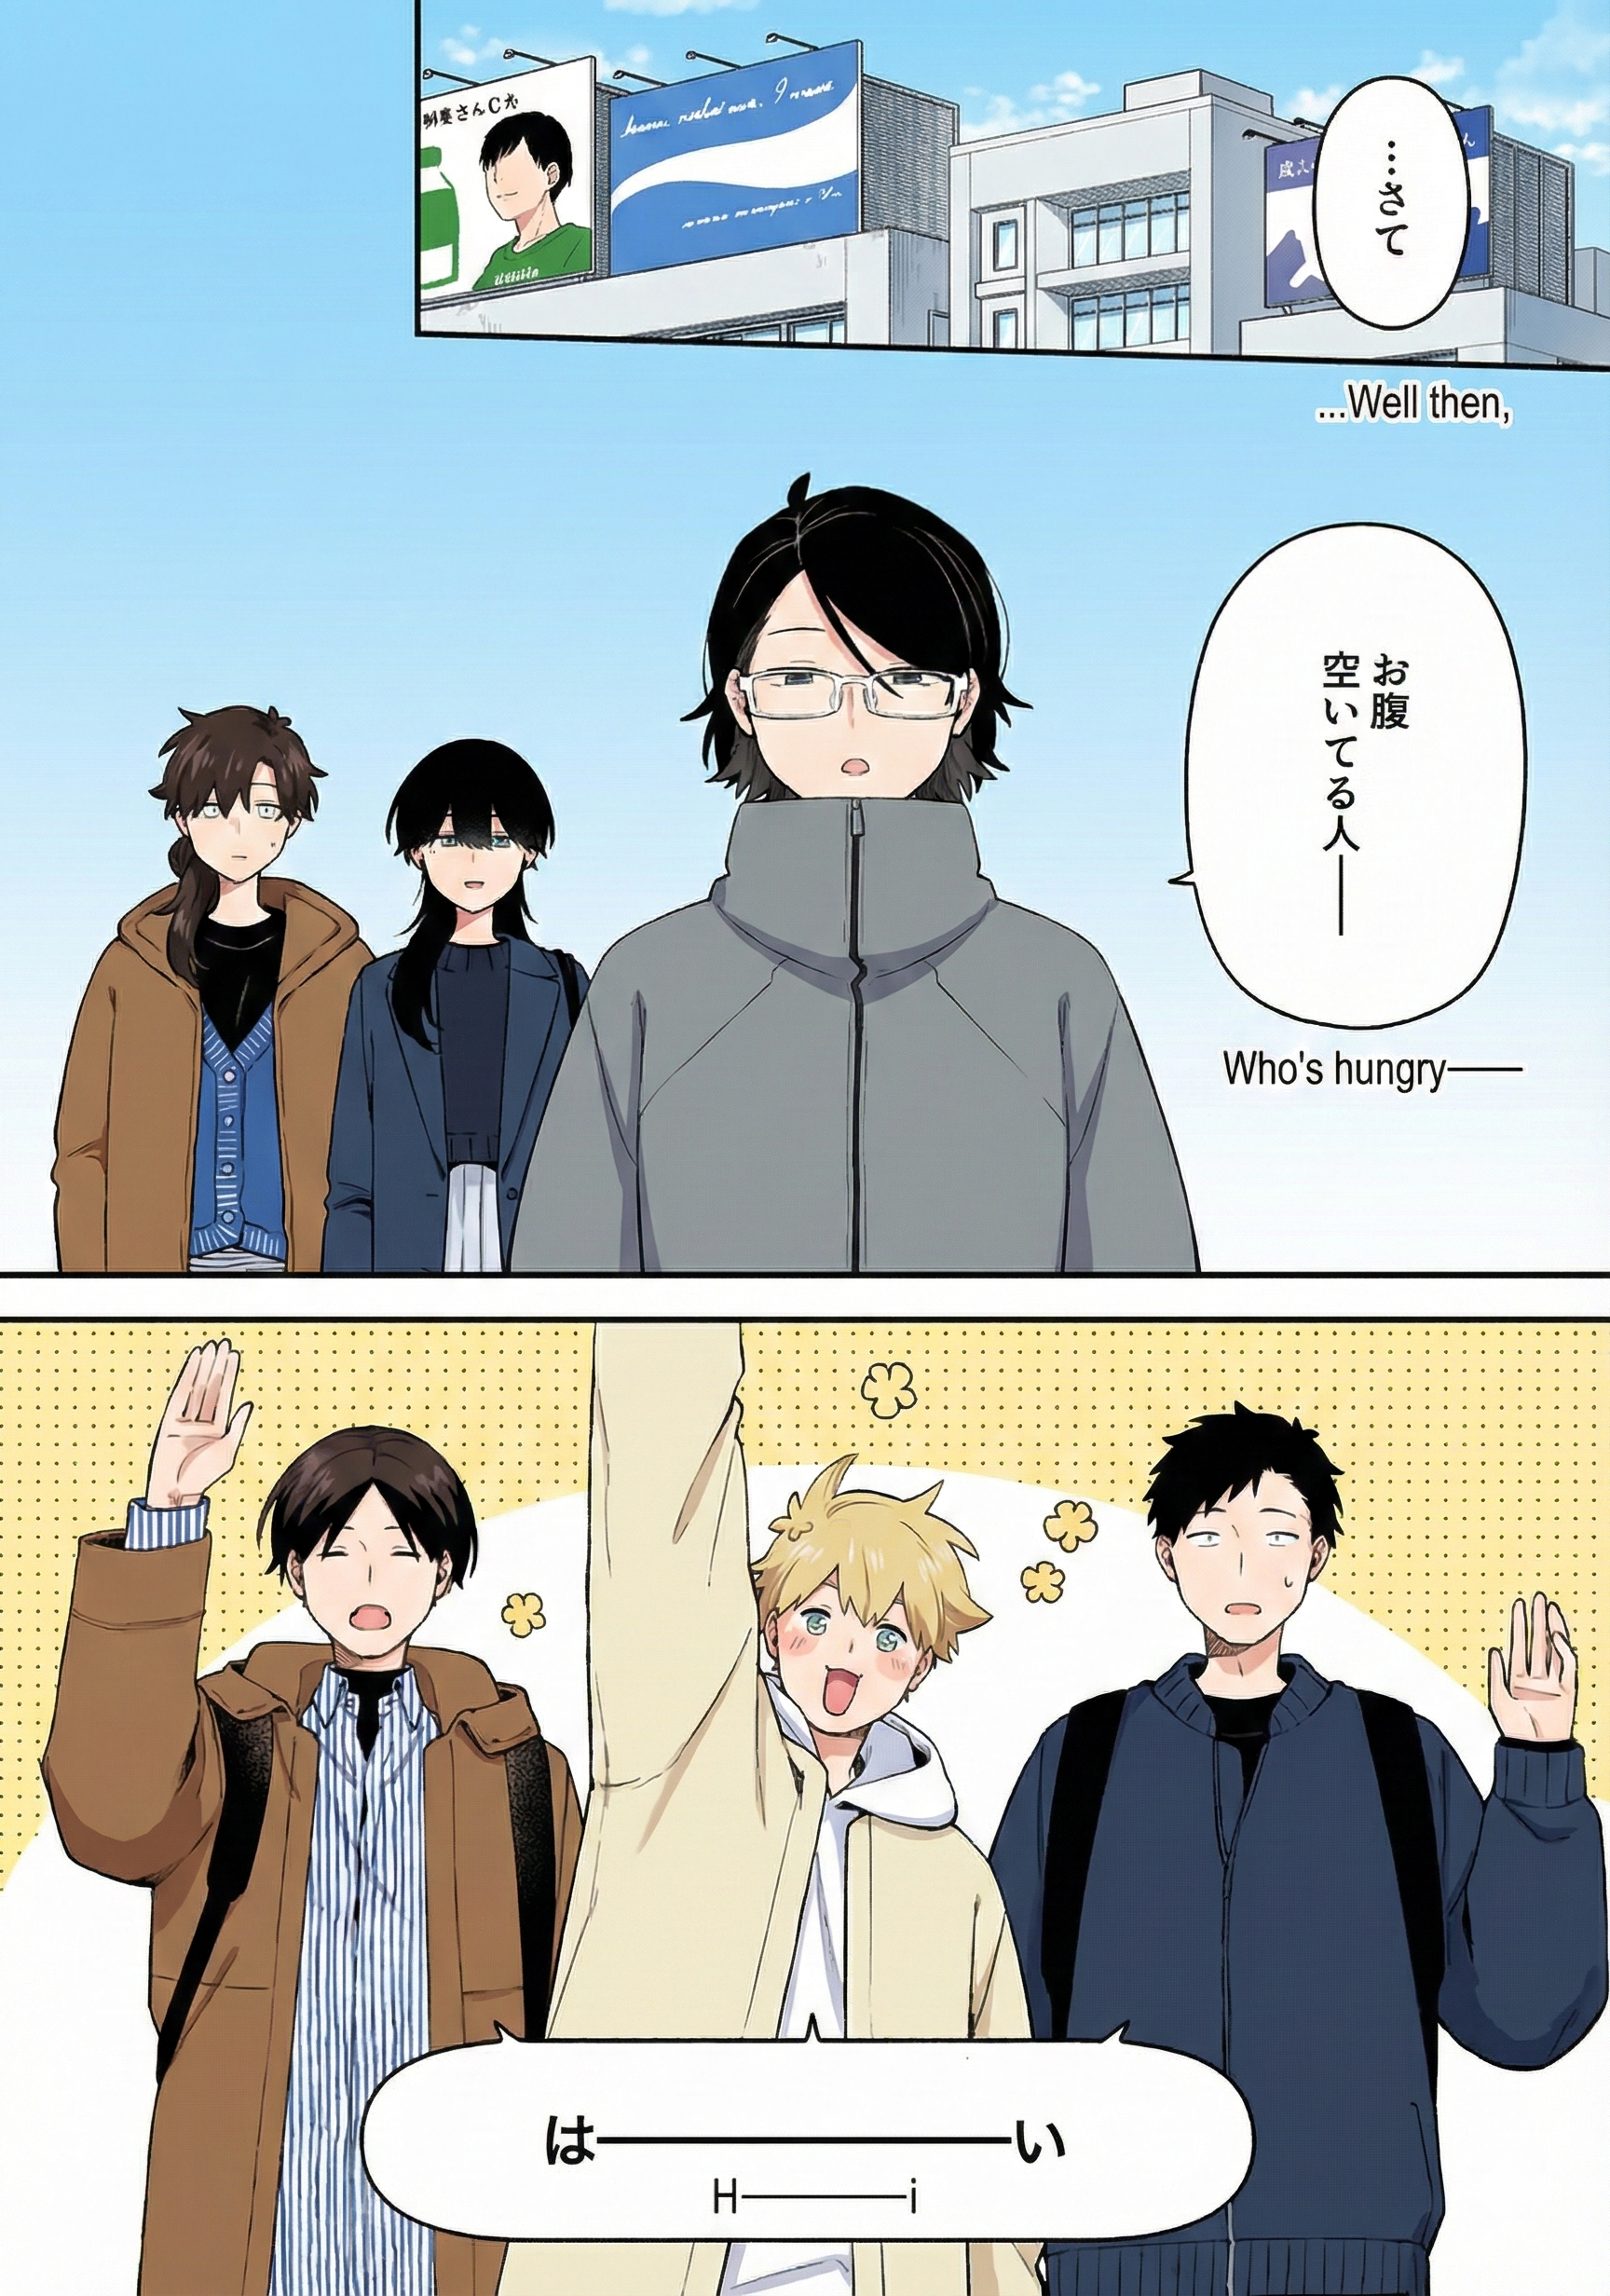
\includegraphics[width=0.7\textwidth]{figure/bilingual_translation.png}
    \caption{이중 언어 표시 결과 예시}
    \label{fig:bilingual}
\end{figure}

이중 언어 표시를 위해 프롬프트에 다음과 같은 지침을 추가한다.

\begin{lstlisting}[caption={이중 언어 표시 프롬프트}]
BILINGUAL DISPLAY MODE:
- Display BOTH Japanese and English in the output image.
- Show the original English text at the TOP of each speech balloon.
- Show the translated English text at the BOTTOM of each speech 
  balloon.
- Both languages should be clearly visible and readable.
- Adjust font sizes if necessary to fit both languages in the 
  speech balloons.
\end{lstlisting}

\subsubsection{향상된 채색 품질}

프롬프트 엔지니어링을 통해 채색 품질을 향상시킬 수 있음을 확인하였다. 특히 다음과 같은 지침을 추가함으로써 그림자와 빛 효과가 개선된 다채로운 채색 결과를 얻을 수 있었다.

\begin{figure}[H]
    \centering
    \includegraphics[width=0.9\textwidth]{figure/enhanced_colorization_comparison.png}
    \caption{향상된 채색 품질 비교}
    \label{fig:enhanced_colorization}
\end{figure}

\begin{lstlisting}[caption={향상된 채색을 위한 프롬프트}]
COLORING REQUIREMENTS:
- Apply vibrant, rich, and diverse colors throughout the entire 
  image.
- Use a colorful and visually appealing palette that brings the 
  manga to life.
- Add depth and dimension with shading and highlights where 
  appropriate.
- Make the coloring look professional and polished like a 
  published color manga.
\end{lstlisting}

Figure~\ref{fig:enhanced_colorization}에서 확인할 수 있듯이, 해당 프롬프트를 추가함으로써 단순한 평면적 채색이 아닌, 입체감 있는 그림자와 하이라이트가 적용된 전문적인 수준의 채색 결과를 얻을 수 있었다.

\subsubsection{웹사이트 배포}

개발된 Nano Manana 시스템은 웹 애플리케이션 형태로 배포되어 누구나 사용할 수 있도록 공개하였다.

\begin{figure}[H]
    \centering
    \includegraphics[width=0.9\textwidth]{figure/nano_manana_web_hero.png}
    \caption{Nano Manana 웹사이트 메인 화면}
    \label{fig:nano_web_hero}
\end{figure}

\begin{figure}[H]
    \centering
    \includegraphics[width=0.9\textwidth]{figure/nano_manana_web_working.png}
    \caption{Nano Manana 웹사이트 작동 화면}
    \label{fig:nano_web_working}
\end{figure}

웹사이트는 \url{https://nano-manana.vercel.app}에서 접근할 수 있다. 사용자는 manga 이미지를 업로드하고 원하는 작업(채색, 번역, 또는 둘 다)을 선택하여 결과를 얻을 수 있다.

\subsection{시도했지만 실패한 방법들}

본 연구 과정에서 일관성 향상과 효율성 개선을 위해 여러 가지 방법을 시도하였으나, 일부는 기대한 성과를 달성하지 못하였다. 이러한 실패 사례들은 향후 연구의 방향을 설정하는 데 중요한 교훈을 제공한다.

\subsubsection{Model Sheet 생성}

캐릭터 일관성 향상과 input token 수 절감을 위해 각 캐릭터의 전신 model sheet를 생성하여 항상 reference로 제공하는 방법을 시도하였다. Model sheet란 각 캐릭터가 정자세로 전신을 보이고 있는 참조 이미지로, 애니메이션이나 게임 제작에서 캐릭터 디자인의 일관성을 유지하기 위해 널리 사용되는 방식이다.

\begin{figure}[H]
    \centering
    \includegraphics[width=0.6\textwidth]{figure/model_sheet_expected.png}
    \caption{기대한 Model Sheet 형태}
    \label{fig:model_sheet_expected}
\end{figure}

여러 manga 페이지를 입력으로 제공하고, 등장하는 모든 캐릭터의 model sheet를 생성하도록 요청하였다. 이상적으로는 Figure~\ref{fig:model_sheet_expected}와 같이 각 캐릭터의 전신이 명확하게 표현된 sheet가 생성되기를 기대하였다.

\begin{lstlisting}[caption={Model Sheet 생성 프롬프트}]
Create a structured character model sheet based strictly on the 
provided black and white manga image. It is absolutely necessary 
that you only extract the specific characters and outfit designs 
actually present in the source photo; do not invent any new 
characters or create any new outfit variations not shown in the 
original image. The final output should be organized into exactly 
two distinct horizontal rows. In the very first top row, arrange 
a black and white model sheet displaying a single, clear 
full-body pose for each unique character found in the input.
\end{lstlisting}

\begin{figure}[H]
    \centering
    \begin{subfigure}[b]{0.3\textwidth}
        \centering
        \includegraphics[width=\textwidth]{figure/model_sheet_failed/ex1.png}
        \caption{실패 사례 1}
    \end{subfigure}
    \hfill
    \begin{subfigure}[b]{0.3\textwidth}
        \centering
        \includegraphics[width=\textwidth]{figure/model_sheet_failed/ex2.png}
        \caption{실패 사례 2}
    \end{subfigure}
    \hfill
    \begin{subfigure}[b]{0.3\textwidth}
        \centering
        \includegraphics[width=\textwidth]{figure/model_sheet_failed/ex3.png}
        \caption{실패 사례 3}
    \end{subfigure}
    \caption{Model Sheet 생성 실패 사례}
    \label{fig:model_sheet_failed}
\end{figure}

그러나 실험 결과, 다음과 같은 문제들이 발생하였다. 첫째, 모델이 입력 이미지에 과도하게 집중하여 model sheet라는 새로운 형태의 출력을 생성하지 못하였다. 둘째, 원본에 등장하지 않는 캐릭터를 임의로 생성하거나, 반대로 실제 등장하는 캐릭터를 파악하지 못하는 경우가 빈번하였다. 이는 현재 생성 모델이 기존 이미지의 특정 부분을 편집하는 작업에는 능숙하지만, 이미지 전체를 새로운 구조로 재구성하는 작업에는 한계가 있음을 시사한다.

\subsubsection{Grid Batch}

일관성 향상과 input token 수 절감을 위해 여러 페이지를 하나의 grid 이미지로 합쳐서 처리하는 방법을 시도하였다. 예를 들어, 2$\times$1, 3$\times$1, 2$\times$2, 3$\times$3 등의 grid로 여러 페이지를 합친 후 한 번에 채색을 요청하는 방식이다.

\begin{figure}[H]
    \centering
    \begin{subfigure}[b]{0.45\textwidth}
        \centering
        \includegraphics[width=\textwidth]{figure/grid_batch_2x1.png}
        \caption{2$\times$1 Grid}
    \end{subfigure}
    \hfill
    \begin{subfigure}[b]{0.45\textwidth}
        \centering
        \includegraphics[width=\textwidth]{figure/grid_batch_3x1.png}
        \caption{3$\times$1 Grid}
    \end{subfigure}
    \caption{Grid Batch 처리 예시 (1)}
    \label{fig:grid_batch_1}
\end{figure}

\begin{figure}[H]
    \centering
    \begin{subfigure}[b]{0.45\textwidth}
        \centering
        \includegraphics[width=\textwidth]{figure/grid_batch_2x2.png}
        \caption{2$\times$2 Grid}
    \end{subfigure}
    \hfill
    \begin{subfigure}[b]{0.45\textwidth}
        \centering
        \includegraphics[width=\textwidth]{figure/grid_batch_3x3.png}
        \caption{3$\times$3 Grid}
    \end{subfigure}
    \caption{Grid Batch 처리 예시 (2)}
    \label{fig:grid_batch_2}
\end{figure}

그러나 이 방법은 두 가지 심각한 문제를 야기하였다.

\begin{figure}[H]
    \centering
    \includegraphics[width=0.8\textwidth]{figure/grid_batch_low_consistency.png}
    \caption{Grid Batch의 낮은 일관성 문제}
    \label{fig:grid_low_consistency}
\end{figure}

첫째, 2$\times$1 grid만 사용해도 캐릭터가 완전히 다른 외모로 채색되거나, 서로 다른 캐릭터들이 동일한 복장을 착용하는 등 일관성이 크게 저하되었다.

\begin{figure}[H]
    \centering
    \begin{subfigure}[b]{0.45\textwidth}
        \centering
        \includegraphics[width=\textwidth]{figure/grid_batch_original_vs_1x1.png}
        \caption{원본 vs 1$\times$1}
    \end{subfigure}
    \hfill
    \begin{subfigure}[b]{0.45\textwidth}
        \centering
        \includegraphics[width=\textwidth]{figure/grid_batch_2x2_vs_3x3.png}
        \caption{2$\times$2 vs 3$\times$3}
    \end{subfigure}
    \caption{Grid 크기에 따른 품질 저하}
    \label{fig:grid_quality}
\end{figure}

둘째, grid 크기가 커질수록 이미지가 전체적으로 흐려지고(blurry), 특히 2$\times$2 이상의 grid에서는 캐릭터의 얼굴이 일그러져 기괴한 형태로 변형되는 현상이 발생하였다. 이는 생성 모델의 해상도 제한과 관련된 것으로 추정된다.

\subsubsection{Bounding Box Identifier}

캐릭터 일관성 향상을 위해 각 캐릭터를 특정 색상의 bounding box로 표시하여 모델이 개별 캐릭터를 명확하게 인식하도록 유도하는 방법을 시도하였다.

\begin{lstlisting}[caption={Bounding Box 프롬프트}]
Colorize this manga page. Maintain consistency of character. 
Maintain speech balloons and texts. Do not modify speech 
balloons and texts. Each character is highlighted by rectangular 
box with specific color. You can figure out each character with 
this box. Remove all the boxes in final result.
\end{lstlisting}

\begin{figure}[H]
    \centering
    \includegraphics[width=0.7\textwidth]{figure/bbox_identifier_fail.png}
    \caption{Bounding Box 제거 실패 사례}
    \label{fig:bbox_fail}
\end{figure}

그러나 프롬프트에서 bounding box를 최종 결과에서 제거하라고 명시적으로 지시했음에도 불구하고, 생성된 이미지에 box가 그대로 남아있는 문제가 발생하였다. 이는 현재 생성 모델이 이미지의 특정 요소를 선택적으로 제거하는 작업에 한계가 있음을 보여준다.

\newpage

% 실험 결과
\section{실험 결과}

\subsection{처리 결과}

Nano Manana 시스템을 사용하여 두 가지 manga 데이터셋에 대해 채색 및 번역 실험을 수행하였다. 상세한 처리 결과는 Appendix A, B, C에 수록하였다.

Appendix A에서는 baseline 시스템(Gemini 웹앱을 사용한 순차적 처리)의 결과를 제시한다. 「合コンに行ったら女がいなかった話」 18페이지에 대한 원본과 채색 결과를 비교하여 확인할 수 있다.

Appendix B에서는 Nano Manana를 사용하여 동일한 manga를 일본어에서 한국어로 번역하고 채색한 결과를 제시한다. Baseline 대비 더 다채로운 색 표현이 이루어졌으나, 일부 페이지에서 원본과 완전히 다른 장면이 생성되는 빈도가 증가하였다.

Appendix C에서는 「神は友達が少ない」를 일본어에서 영어로 번역하고 채색한 결과를 제시한다. 이 데이터셋에서는 캐릭터의 일관성이 특히 잘 유지되었는데, 이는 Genshin Impact라는 게임의 캐릭터가 인터넷에 널리 알려져 있어 모델의 사전 학습에 많이 포함되었기 때문으로 추정된다.

\subsection{Nano Manana의 한계}

실험 과정에서 Nano Manana 시스템의 몇 가지 한계점이 발견되었다. 이러한 한계는 주로 기반 모델인 Gemini Imagen 3의 특성에 기인한다.

\subsubsection{완전히 새로운 스타일이 생성되는 문제}

\begin{figure}[H]
    \centering
    \includegraphics[width=0.9\textwidth]{figure/pixiv1_original_vs_manana_ct_b5/p13.png}
    \caption{원본과 완전히 다른 스타일로 생성된 사례}
    \label{fig:different_style}
\end{figure}

일부 페이지에서 같은 장소와 내용임에도 불구하고 완전히 다른 스타일의 인물이 그려지는 현상이 발생하였다. 흥미로운 점은 번역 대상 언어에 따라 생성되는 스타일이 달라진다는 것이다. 한국어로 번역을 요청하면 한국 웹툰 스타일의 그림이 생성되는 경향이 있었고, 영어로 번역을 요청하면 서양 cartoon 느낌의 그림이 생성되는 경향이 있었다. 프롬프트에서 새로운 스타일을 생성하지 말라고 강조해도 간헐적으로 이러한 현상이 발생하였다.

\subsubsection{완전히 다른 장면이 생성되는 문제}

Figure~\ref{fig:different_style}에서 확인할 수 있듯이, 일부 경우에서 원본과 장면 자체가 완전히 달라지는 문제가 발생하였다. 번역된 텍스트의 내용을 확인하면 상황과 맥락도 원본과 전혀 다르게 생성되어 있음을 알 수 있다. 이는 생성 모델이 이미지를 편집하는 것이 아니라 완전히 새로운 이미지를 생성해버리는 것으로, manga 채색 및 번역의 핵심 요구사항인 원본 보존에 심각한 문제가 된다.

\subsubsection{다른 비율로 생성되는 문제}

\begin{figure}[H]
    \centering
    \includegraphics[width=0.7\textwidth]{figure/nano_manana_fail_different_aspect_ratio.png}
    \caption{원본과 다른 비율로 생성된 사례}
    \label{fig:different_ratio}
\end{figure}

프롬프트에서 원본 이미지의 비율(aspect ratio)을 명확하게 명시했음에도 불구하고, 생성된 이미지가 완전히 다른 비율로 출력되는 경우가 있었다. 이러한 문제들은 모두 Gemini Imagen 3 모델 자체의 특성에서 비롯되는 것으로, 프롬프트 엔지니어링만으로는 완전히 해결하기 어려운 한계가 있다.

\subsection{API 동작 비용}

Nano Manana 시스템의 API 사용량과 비용을 분석하였다.

\begin{figure}[H]
    \centering
    \includegraphics[width=0.9\textwidth]{figure/nano_manana_api_token_chart.png}
    \caption{API Token 사용량 분포}
    \label{fig:api_token_chart}
\end{figure}

\begin{table}[H]
    \centering
    \caption{API Token 및 비용 통계}
    \label{tab:api_stats}
    \begin{tabular}{lccc}
        \toprule
        \textbf{항목} & \textbf{평균} & \textbf{표준편차} & \textbf{합계} \\
        \midrule
        Prompt Text Token & 207.56 & 162.64 & 22,832 \\
        Prompt Image Token & 602.78 & 511.58 & 66,306 \\
        Thought Token & 611.95 & 348.88 & 67,315 \\
        Candidate Image Token & 1,120.00 & 0.00 & 123,200 \\
        Total Token & 2,542.30 & 836.15 & 279,653 \\
        \midrule
        Prompt Text Price (\$) & 0.00 & 0.00 & 0.05 \\
        Prompt Image Price (\$) & 0.00 & 0.00 & 0.13 \\
        Thought Price (\$) & 0.01 & 0.00 & 0.81 \\
        Candidate Image Price (\$) & 0.13 & 0.00 & 14.78 \\
        Total Price (\$) & 0.14 & 0.00 & 15.77 \\
        \bottomrule
    \end{tabular}
\end{table}

전체 프로젝트 진행 과정에서 총 155회의 API 요청이 수행되었으며, 총 API 비용은 약 \$15.77(한화 약 33,372원)이 소요되었다. API 비용의 대부분은 candidate image token(생성된 이미지)에서 발생하였으며, 이는 전체 비용의 약 94\%를 차지한다.

\subsection{소스코드 통계}

\begin{figure}[H]
    \centering
    \includegraphics[width=0.8\textwidth]{figure/git_contribution_stats.png}
    \caption{Git Contribution 통계}
    \label{fig:git_stats}
\end{figure}

본 연구를 위해 작성된 소스코드의 통계는 다음과 같다. 총 23,130줄의 코드가 추가되었으며, 2,740줄의 코드가 삭제되었다. 이는 웹 애플리케이션, API 통신, batch 처리 로직, 프롬프트 관리 등 전체 시스템 구축에 필요한 코드를 포함한다.

\newpage

% 결론
\section{결론}

본 연구에서는 manga의 채색과 번역을 자동화하면서 전체 페이지에 걸쳐 배경과 캐릭터의 일관성을 유지하는 Nano Manana 시스템을 개발하였다. 주요 연구 성과와 결론은 다음과 같다.

첫째, 대다수의 경우에서 높은 품질의 채색 결과를 생성할 수 있었다. 프롬프트 엔지니어링을 통해 그림자와 빛 효과가 향상된 다채로운 채색이 가능하며, baseline 시스템 대비 더 전문적인 수준의 결과물을 얻을 수 있었다.

둘째, 이중 언어 번역과 의성어, 의태어, 물체 내 텍스트를 포함한 포괄적인 번역이 가능하다. 기존 연구들이 텍스트만 번역하는 것과 달리, Nano Manana는 역본 작업과 식질 작업을 통합하여 end-to-end로 번역된 manga 이미지를 생성한다.

셋째, batch 처리 구조를 통해 baseline 대비 번역 작업에서 최대 10배, 채색 작업에서 최대 5배의 속도 향상을 달성하였다. 채색의 경우 reference 이미지 최대 개수가 5개로 제한되어 있어 5배가 상한이다.

그러나 본 시스템에는 몇 가지 한계가 존재한다. 높은 빈도로 원본에 없는 장면이 생성되거나 캐릭터 일관성이 무너지는 경우가 관찰되었다. 이러한 문제는 기반 모델인 Gemini Imagen 3의 특성에 기인하며, model sheet 생성, grid batch, bounding box identifier 등 여러 방법을 시도하였으나 근본적인 해결에는 이르지 못하였다.

당장의 해결책으로는 사용자 확인 기반의 품질 관리 시스템을 제안한다. 생성된 각 페이지를 사용자가 확인하여 accept 또는 reject를 선택하고, reject된 페이지는 자동으로 재생성(rerun)하는 방식이다. 이를 통해 최종 결과물의 품질을 보장하면서도 자동화의 이점을 유지할 수 있다.

향후 연구로는 캐릭터 인식 및 추적 기술을 도입하여 일관성 유지 능력을 향상시키는 방안, 그리고 사용자 피드백을 학습에 반영하는 강화학습 기반 접근법 등을 고려할 수 있다.

\newpage

% 참고문헌
\bibliographystyle{plain}
\begin{thebibliography}{9}

\bibitem{mangadit}
Qiu, Q., Mao, J., Masui, K., \& Wang, X.,
\textit{MangaDiT: Reference-Guided Line Art Colorization with Hierarchical Attention in Diffusion Transformers},
arXiv preprint arXiv:2508.09709, 2025.

\bibitem{manganinja}
Liu, Z., Cheng, K. L., Chen, X., Xiao, J., Ouyang, H., Zhu, K., Liu, Y., Shen, Y., Chen, Q., \& Luo, P.,
\textit{MangaNinja: Line Art Colorization with Precise Reference Following},
arXiv preprint arXiv:2501.08332, 2025.

\bibitem{mangamllm}
Lippmann, P., Skublicki, K., Tanner, J., Ishiwatari, S., \& Yang, J.,
\textit{Context-Informed Machine Translation of Manga using Multimodal Large Language Models},
Proceedings of the 31st International Conference on Computational Linguistics (COLING), pages 3444--3464, Abu Dhabi, UAE, 2025.

\bibitem{pixiv_goukon}
蒼川なな (Aokawa Nana),
\textit{「合コンに行ったら女がいなかった話」(How I Attended an All-Guy's Mixer)},
pixiv, 2025.
\url{https://www.pixiv.net/en/artworks/136886858}

\bibitem{pixiv_kami}
ピノ/エス (Pino/Esu),
\textit{「神は友達が少ない」(God Has Few Friends)},
pixiv, 2023.
\url{https://www.pixiv.net/en/artworks/107422372}

\bibitem{galleryDL}
mikf,
\textit{gallery-dl: Command-line program to download image galleries and collections from several image hosting sites},
GitHub, 2025.
\url{https://github.com/mikf/gallery-dl}

\end{thebibliography}

\newpage

% Appendix
\appendix

\section{Baseline 처리 결과}
\label{appendix:baseline}

본 Appendix에서는 baseline 시스템(Gemini 웹앱을 사용한 순차적 처리)의 결과를 제시한다. 「合コンに行ったら女がいなかった話」 18페이지에 대한 원본과 채색 결과를 비교할 수 있다.

\begin{figure}[H]
    \centering
    \begin{subfigure}[b]{0.45\textwidth}
        \centering
        \includegraphics[width=\textwidth]{figure/pixiv1_original_vs_nbp-base/p0.png}
        \caption{Page 0}
    \end{subfigure}
    \hfill
    \begin{subfigure}[b]{0.45\textwidth}
        \centering
        \includegraphics[width=\textwidth]{figure/pixiv1_original_vs_nbp-base/p1.png}
        \caption{Page 1}
    \end{subfigure}
\end{figure}

\begin{figure}[H]
    \centering
    \begin{subfigure}[b]{0.45\textwidth}
        \centering
        \includegraphics[width=\textwidth]{figure/pixiv1_original_vs_nbp-base/p2.png}
        \caption{Page 2}
    \end{subfigure}
    \hfill
    \begin{subfigure}[b]{0.45\textwidth}
        \centering
        \includegraphics[width=\textwidth]{figure/pixiv1_original_vs_nbp-base/p3.png}
        \caption{Page 3}
    \end{subfigure}
\end{figure}

\begin{figure}[H]
    \centering
    \begin{subfigure}[b]{0.45\textwidth}
        \centering
        \includegraphics[width=\textwidth]{figure/pixiv1_original_vs_nbp-base/p4.png}
        \caption{Page 4}
    \end{subfigure}
    \hfill
    \begin{subfigure}[b]{0.45\textwidth}
        \centering
        \includegraphics[width=\textwidth]{figure/pixiv1_original_vs_nbp-base/p5.png}
        \caption{Page 5}
    \end{subfigure}
\end{figure}

\begin{figure}[H]
    \centering
    \begin{subfigure}[b]{0.45\textwidth}
        \centering
        \includegraphics[width=\textwidth]{figure/pixiv1_original_vs_nbp-base/p6.png}
        \caption{Page 6}
    \end{subfigure}
    \hfill
    \begin{subfigure}[b]{0.45\textwidth}
        \centering
        \includegraphics[width=\textwidth]{figure/pixiv1_original_vs_nbp-base/p7.png}
        \caption{Page 7}
    \end{subfigure}
\end{figure}

\begin{figure}[H]
    \centering
    \begin{subfigure}[b]{0.45\textwidth}
        \centering
        \includegraphics[width=\textwidth]{figure/pixiv1_original_vs_nbp-base/p8.png}
        \caption{Page 8}
    \end{subfigure}
    \hfill
    \begin{subfigure}[b]{0.45\textwidth}
        \centering
        \includegraphics[width=\textwidth]{figure/pixiv1_original_vs_nbp-base/p9.png}
        \caption{Page 9}
    \end{subfigure}
\end{figure}

\begin{figure}[H]
    \centering
    \begin{subfigure}[b]{0.45\textwidth}
        \centering
        \includegraphics[width=\textwidth]{figure/pixiv1_original_vs_nbp-base/p10.png}
        \caption{Page 10}
    \end{subfigure}
    \hfill
    \begin{subfigure}[b]{0.45\textwidth}
        \centering
        \includegraphics[width=\textwidth]{figure/pixiv1_original_vs_nbp-base/p11.png}
        \caption{Page 11}
    \end{subfigure}
\end{figure}

\begin{figure}[H]
    \centering
    \begin{subfigure}[b]{0.45\textwidth}
        \centering
        \includegraphics[width=\textwidth]{figure/pixiv1_original_vs_nbp-base/p12.png}
        \caption{Page 12}
    \end{subfigure}
    \hfill
    \begin{subfigure}[b]{0.45\textwidth}
        \centering
        \includegraphics[width=\textwidth]{figure/pixiv1_original_vs_nbp-base/p13.png}
        \caption{Page 13}
    \end{subfigure}
\end{figure}

\begin{figure}[H]
    \centering
    \begin{subfigure}[b]{0.45\textwidth}
        \centering
        \includegraphics[width=\textwidth]{figure/pixiv1_original_vs_nbp-base/p14.png}
        \caption{Page 14}
    \end{subfigure}
    \hfill
    \begin{subfigure}[b]{0.45\textwidth}
        \centering
        \includegraphics[width=\textwidth]{figure/pixiv1_original_vs_nbp-base/p15.png}
        \caption{Page 15}
    \end{subfigure}
\end{figure}

\begin{figure}[H]
    \centering
    \begin{subfigure}[b]{0.45\textwidth}
        \centering
        \includegraphics[width=\textwidth]{figure/pixiv1_original_vs_nbp-base/p16.png}
        \caption{Page 16}
    \end{subfigure}
    \hfill
    \begin{subfigure}[b]{0.45\textwidth}
        \centering
        \includegraphics[width=\textwidth]{figure/pixiv1_original_vs_nbp-base/p17.png}
        \caption{Page 17}
    \end{subfigure}
    \caption{Baseline 처리 결과: 「合コンに行ったら女がいなかった話」 원본 vs 채색}
    \label{fig:appendix_baseline}
\end{figure}

\newpage

\section{Nano Manana 일본어 → 한국어 처리 결과}
\label{appendix:nano_jp_kr}

본 Appendix에서는 Nano Manana를 사용하여 「合コンに行ったら女がいなかった話」를 일본어에서 한국어로 번역하고 채색한 결과를 제시한다. Baseline 대비 더 다채로운 색 표현이 이루어졌으나, 일부 페이지에서 원본과 완전히 다른 장면이 생성되는 빈도가 증가하였다.

\begin{figure}[H]
    \centering
    \begin{subfigure}[b]{0.45\textwidth}
        \centering
        \includegraphics[width=\textwidth]{figure/pixiv1_original_vs_manana_ct_b5/p0.png}
        \caption{Page 0}
    \end{subfigure}
    \hfill
    \begin{subfigure}[b]{0.45\textwidth}
        \centering
        \includegraphics[width=\textwidth]{figure/pixiv1_original_vs_manana_ct_b5/p1.png}
        \caption{Page 1}
    \end{subfigure}
\end{figure}

\begin{figure}[H]
    \centering
    \begin{subfigure}[b]{0.45\textwidth}
        \centering
        \includegraphics[width=\textwidth]{figure/pixiv1_original_vs_manana_ct_b5/p2.png}
        \caption{Page 2}
    \end{subfigure}
    \hfill
    \begin{subfigure}[b]{0.45\textwidth}
        \centering
        \includegraphics[width=\textwidth]{figure/pixiv1_original_vs_manana_ct_b5/p3.png}
        \caption{Page 3}
    \end{subfigure}
\end{figure}

\begin{figure}[H]
    \centering
    \begin{subfigure}[b]{0.45\textwidth}
        \centering
        \includegraphics[width=\textwidth]{figure/pixiv1_original_vs_manana_ct_b5/p4.png}
        \caption{Page 4}
    \end{subfigure}
    \hfill
    \begin{subfigure}[b]{0.45\textwidth}
        \centering
        \includegraphics[width=\textwidth]{figure/pixiv1_original_vs_manana_ct_b5/p5.png}
        \caption{Page 5}
    \end{subfigure}
\end{figure}

\begin{figure}[H]
    \centering
    \begin{subfigure}[b]{0.45\textwidth}
        \centering
        \includegraphics[width=\textwidth]{figure/pixiv1_original_vs_manana_ct_b5/p6.png}
        \caption{Page 6}
    \end{subfigure}
    \hfill
    \begin{subfigure}[b]{0.45\textwidth}
        \centering
        \includegraphics[width=\textwidth]{figure/pixiv1_original_vs_manana_ct_b5/p7.png}
        \caption{Page 7}
    \end{subfigure}
\end{figure}

\begin{figure}[H]
    \centering
    \begin{subfigure}[b]{0.45\textwidth}
        \centering
        \includegraphics[width=\textwidth]{figure/pixiv1_original_vs_manana_ct_b5/p8.png}
        \caption{Page 8}
    \end{subfigure}
    \hfill
    \begin{subfigure}[b]{0.45\textwidth}
        \centering
        \includegraphics[width=\textwidth]{figure/pixiv1_original_vs_manana_ct_b5/p9.png}
        \caption{Page 9}
    \end{subfigure}
\end{figure}

\begin{figure}[H]
    \centering
    \begin{subfigure}[b]{0.45\textwidth}
        \centering
        \includegraphics[width=\textwidth]{figure/pixiv1_original_vs_manana_ct_b5/p10.png}
        \caption{Page 10}
    \end{subfigure}
    \hfill
    \begin{subfigure}[b]{0.45\textwidth}
        \centering
        \includegraphics[width=\textwidth]{figure/pixiv1_original_vs_manana_ct_b5/p11.png}
        \caption{Page 11}
    \end{subfigure}
\end{figure}

\begin{figure}[H]
    \centering
    \begin{subfigure}[b]{0.45\textwidth}
        \centering
        \includegraphics[width=\textwidth]{figure/pixiv1_original_vs_manana_ct_b5/p12.png}
        \caption{Page 12}
    \end{subfigure}
    \hfill
    \begin{subfigure}[b]{0.45\textwidth}
        \centering
        \includegraphics[width=\textwidth]{figure/pixiv1_original_vs_manana_ct_b5/p13.png}
        \caption{Page 13}
    \end{subfigure}
\end{figure}

\begin{figure}[H]
    \centering
    \begin{subfigure}[b]{0.45\textwidth}
        \centering
        \includegraphics[width=\textwidth]{figure/pixiv1_original_vs_manana_ct_b5/p14.png}
        \caption{Page 14}
    \end{subfigure}
    \hfill
    \begin{subfigure}[b]{0.45\textwidth}
        \centering
        \includegraphics[width=\textwidth]{figure/pixiv1_original_vs_manana_ct_b5/p15.png}
        \caption{Page 15}
    \end{subfigure}
\end{figure}

\begin{figure}[H]
    \centering
    \begin{subfigure}[b]{0.45\textwidth}
        \centering
        \includegraphics[width=\textwidth]{figure/pixiv1_original_vs_manana_ct_b5/p16.png}
        \caption{Page 16}
    \end{subfigure}
    \hfill
    \begin{subfigure}[b]{0.45\textwidth}
        \centering
        \includegraphics[width=\textwidth]{figure/pixiv1_original_vs_manana_ct_b5/p17.png}
        \caption{Page 17}
    \end{subfigure}
\end{figure}

\begin{figure}[H]
    \centering
    \includegraphics[width=0.45\textwidth]{figure/pixiv1_original_vs_manana_ct_b5/p18.png}
    \caption{Nano Manana 일본어→한국어 처리 결과: 「合コンに行ったら女がいなかった話」}
    \label{fig:appendix_nano_jp_kr}
\end{figure}

\newpage

\section{Nano Manana 일본어 → 영어 처리 결과}
\label{appendix:nano_jp_en}

본 Appendix에서는 Nano Manana를 사용하여 「神は友達が少ない」를 일본어에서 영어로 번역하고 채색한 결과를 제시한다. 이 데이터셋에서는 캐릭터의 일관성이 특히 잘 유지되었는데, 이는 Genshin Impact라는 게임의 캐릭터가 인터넷에 널리 알려져 있어 모델의 사전 학습에 많이 포함되었기 때문으로 추정된다.

\begin{figure}[H]
    \centering
    \begin{subfigure}[b]{0.45\textwidth}
        \centering
        \includegraphics[width=\textwidth]{figure/pixiv2_original_vs_manana_ct_b5/p0.png}
        \caption{Page 0}
    \end{subfigure}
    \hfill
    \begin{subfigure}[b]{0.45\textwidth}
        \centering
        \includegraphics[width=\textwidth]{figure/pixiv2_original_vs_manana_ct_b5/p1.png}
        \caption{Page 1}
    \end{subfigure}
\end{figure}

\begin{figure}[H]
    \centering
    \begin{subfigure}[b]{0.45\textwidth}
        \centering
        \includegraphics[width=\textwidth]{figure/pixiv2_original_vs_manana_ct_b5/p2.png}
        \caption{Page 2}
    \end{subfigure}
    \hfill
    \begin{subfigure}[b]{0.45\textwidth}
        \centering
        \includegraphics[width=\textwidth]{figure/pixiv2_original_vs_manana_ct_b5/p3.png}
        \caption{Page 3}
    \end{subfigure}
\end{figure}

\begin{figure}[H]
    \centering
    \begin{subfigure}[b]{0.45\textwidth}
        \centering
        \includegraphics[width=\textwidth]{figure/pixiv2_original_vs_manana_ct_b5/p4.png}
        \caption{Page 4}
    \end{subfigure}
    \hfill
    \begin{subfigure}[b]{0.45\textwidth}
        \centering
        \includegraphics[width=\textwidth]{figure/pixiv2_original_vs_manana_ct_b5/p5.png}
        \caption{Page 5}
    \end{subfigure}
\end{figure}

\begin{figure}[H]
    \centering
    \begin{subfigure}[b]{0.45\textwidth}
        \centering
        \includegraphics[width=\textwidth]{figure/pixiv2_original_vs_manana_ct_b5/p6.png}
        \caption{Page 6}
    \end{subfigure}
    \hfill
    \begin{subfigure}[b]{0.45\textwidth}
        \centering
        \includegraphics[width=\textwidth]{figure/pixiv2_original_vs_manana_ct_b5/p7.png}
        \caption{Page 7}
    \end{subfigure}
\end{figure}

\begin{figure}[H]
    \centering
    \begin{subfigure}[b]{0.45\textwidth}
        \centering
        \includegraphics[width=\textwidth]{figure/pixiv2_original_vs_manana_ct_b5/p8.png}
        \caption{Page 8}
    \end{subfigure}
    \hfill
    \begin{subfigure}[b]{0.45\textwidth}
        \centering
        \includegraphics[width=\textwidth]{figure/pixiv2_original_vs_manana_ct_b5/p9.png}
        \caption{Page 9}
    \end{subfigure}
\end{figure}

\begin{figure}[H]
    \centering
    \begin{subfigure}[b]{0.45\textwidth}
        \centering
        \includegraphics[width=\textwidth]{figure/pixiv2_original_vs_manana_ct_b5/p10.png}
        \caption{Page 10}
    \end{subfigure}
    \hfill
    \begin{subfigure}[b]{0.45\textwidth}
        \centering
        \includegraphics[width=\textwidth]{figure/pixiv2_original_vs_manana_ct_b5/p11.png}
        \caption{Page 11}
    \end{subfigure}
\end{figure}

\begin{figure}[H]
    \centering
    \begin{subfigure}[b]{0.45\textwidth}
        \centering
        \includegraphics[width=\textwidth]{figure/pixiv2_original_vs_manana_ct_b5/p12.png}
        \caption{Page 12}
    \end{subfigure}
    \hfill
    \begin{subfigure}[b]{0.45\textwidth}
        \centering
        \includegraphics[width=\textwidth]{figure/pixiv2_original_vs_manana_ct_b5/p13.png}
        \caption{Page 13}
    \end{subfigure}
\end{figure}

\begin{figure}[H]
    \centering
    \begin{subfigure}[b]{0.45\textwidth}
        \centering
        \includegraphics[width=\textwidth]{figure/pixiv2_original_vs_manana_ct_b5/p14.png}
        \caption{Page 14}
    \end{subfigure}
    \hfill
    \begin{subfigure}[b]{0.45\textwidth}
        \centering
        \includegraphics[width=\textwidth]{figure/pixiv2_original_vs_manana_ct_b5/p15.png}
        \caption{Page 15}
    \end{subfigure}
    \caption{Nano Manana 일본어→영어 처리 결과: 「神は友達が少ない」}
    \label{fig:appendix_nano_jp_en}
\end{figure}

\end{document}